%-------------------------------------------------------
\section{The Importance of Capital}
%-------------------------------------------------------

\begin{frame}

\begin{center}
{\LARGE The Importance of Capital}
\end{center}

\end{frame}

%-------------------------------------------------------

%-------------------------------------------------------

\begin{frame}{Firm balance sheet}

A firm's balance sheet has two sides
	\begin{itemize}
	\item	Assets: Cash, intellectual property, inventory, receivables, machinery, trucks, real estate\ldots
	\item	Liabilities: Bank loans, commercial paper, trade credit, long term debt/bonds, capital
	\end{itemize}
\vspace{2mm}
If a firm's assets $>$ liabilities (\emph{excluding capital}) then we say it is `solvent'
	\begin{itemize}
	\item	Capital $\approx$ buffer of asset value over obligations to \textit{external creditors}
	\item	Simplifying somewhat, it comprises equity and retained earnings
	\item	Natural to think of it as liabilities \textit{to the bank's owners} (shareholders)
	\end{itemize}

\end{frame}

%-------------------------------------------------------

%-------------------------------------------------------

\begin{frame}{Bank balance sheet}

A \textbf{bank} balance sheet also has two sides
	\begin{itemize}
	\item	Assets: Traditionally predominantly loans (also securities, cash etc.)
	\item	Liabilities: Deposits, wholesale funding, bonds, \textbf{capital}
	\end{itemize}
\vspace{2mm}
Other than the composition of the balance sheet, the essential logic of a bank balance sheet is the same as in the firm case
	\begin{itemize}
	\item	The `other than' is obviously very important!
	\end{itemize} 
\vspace{2mm}
Confusing terminology: People (and I will) often refer to the bank's liabilities as excluding equity
	\begin{itemize}
	\item	Under this relabeling\ldots
	\vspace{1mm}
	\item[]	\centering \textcolor{red}{solvency $\Leftrightarrow$ (assets $\geq$ `liabilities') $\Leftrightarrow$ capital $>0$}
	\end{itemize}

\end{frame}

%-------------------------------------------------------

%-------------------------------------------------------

\begin{frame}{Bank balance sheet}

\begin{figure}
\begin{center}

\resizebox{0.30\textwidth}{!}{%
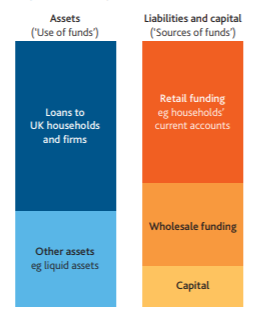
\includegraphics{Figures/simplified_bs.png}
}

\caption{\label{fig:L4_simplified_bs} Simplified bank balance sheet. Source: \href{https://www.bankofengland.co.uk/-/media/boe/files/quarterly-bulletin/2013/bank-capital-and-liquidity.pdf}{Bank of England - Farag (2013)}}

\end{center}
\end{figure}

\end{frame}

%-------------------------------------------------------

%-------------------------------------------------------

\begin{frame}{Composition of assets}

\begin{figure}
\begin{center}

\resizebox{0.70\textwidth}{!}{%
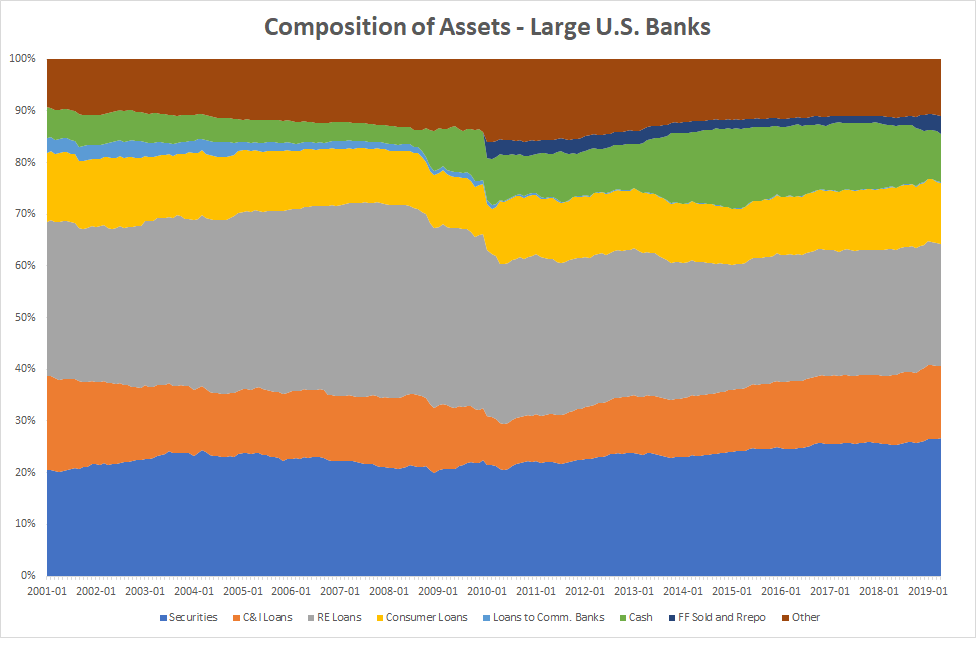
\includegraphics{Figures/Asset_composition_large_banks.png}
}

\caption{\label{fig:L4_Asset_composition_large_banks} Asset composition of large U.S. banks (percent). Source: \href{https://www.federalreserve.gov/releases/h8/current/default.htm}{Federal Reserve table H.8}}

\end{center}
\end{figure}

\end{frame}

%-------------------------------------------------------

%-------------------------------------------------------

\begin{frame}{Composition of liabilities}

\begin{figure}
\begin{center}

\resizebox{0.70\textwidth}{!}{%
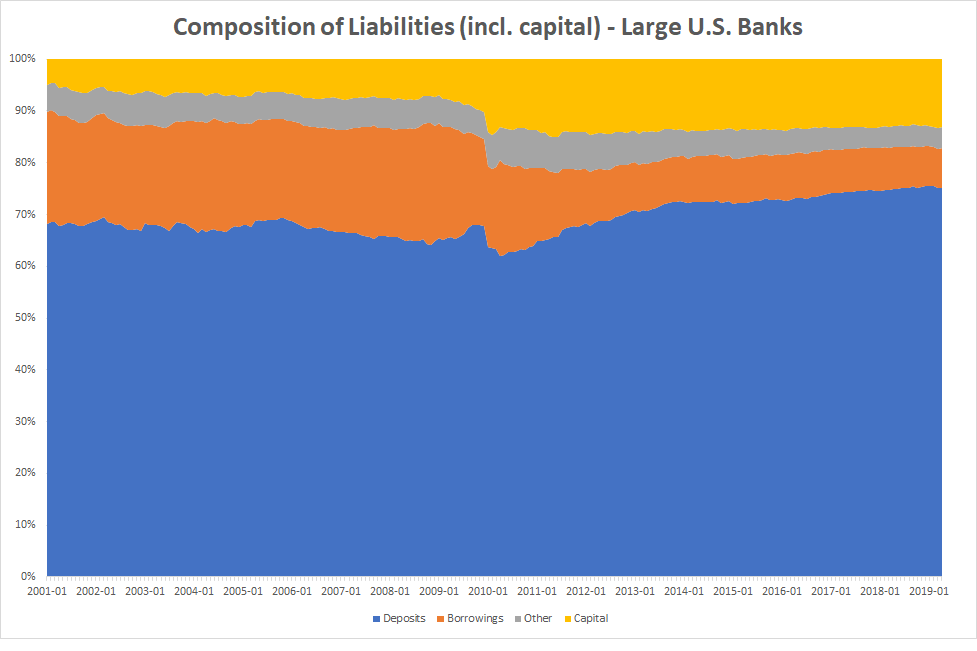
\includegraphics{Figures/Liability_composition_large_banks.png}
}

\caption{\label{fig:L4_Liability_composition_large_banks} Liability (including capital) composition of large U.S. banks (percent). Source: \href{https://www.federalreserve.gov/releases/h8/current/default.htm}{Federal Reserve table H.8}}

\end{center}
\end{figure}

\end{frame}

%-------------------------------------------------------

%-------------------------------------------------------

\begin{frame}{Loans vs. deposits}

\begin{figure}
\begin{center}

\resizebox{0.60\textwidth}{!}{%
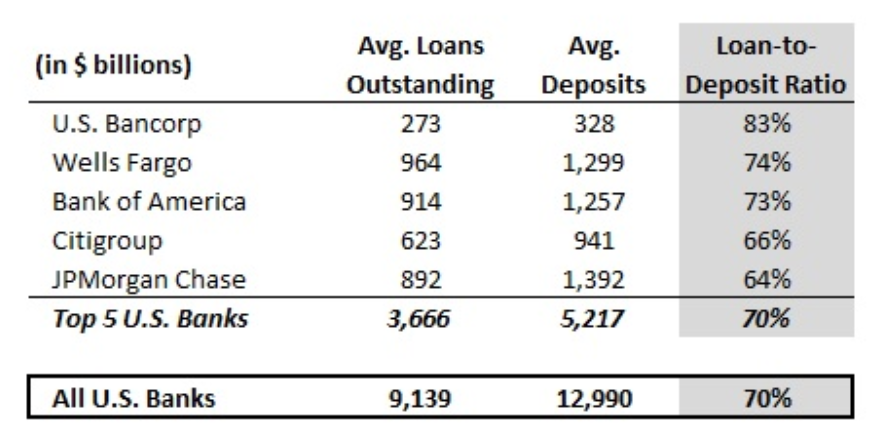
\includegraphics{Figures/2017_loan_to_dep_ratio.png}
}

\caption{\label{fig:L4_2017_loan_to_dep_ratio} Loan to deposit ratios ($2017Q1$). Source: \href{https://www.forbes.com/sites/greatspeculations/2017/06/13/loan-to-deposit-ratios-for-largest-u-s-banks-show-signs-of-recovery-in-q1/\#5d0aa40b12f4}{Forbes (2017)}}

\end{center}
\end{figure}

%Loan-to-deposit ratios (LDRs) across the banking industry have declined steadily since 2010, but some of the largest U.S. banks witnessed a slight uptick in this key metric for Q1 2017 as loan growth outpaced deposit growth. The LDR ratios for the 5 largest banks ranges from around 65\% for JPMorgan Chase and Citigroup to almost 85\% for U.S. Bancorp. The significantly diversified business model for JPMorgan as well as Citigroup (which includes a large custody banking division for both of them) is primarily responsible for their relatively low LDR figures, while U.S. Bancorp’s traditional loans-and-deposits business model explains its higher LDR figure.

%The loan-to-deposit ratio is the ratio of a bank’s total outstanding loans for a period to its total deposit balance over the same period. So an LDR figure of 100\% indicates that a bank lends a dollar to customers for every dollar that it brings in as deposits. But this also means that the bank doesn’t have significant cash on hand for contingencies. A combination of prudence and regulatory requirements suggests that for a traditional bank, the LDR should be around 80-90\%. With a business model that relies heavily on traditional loans-and-deposits services, U.S. Bancorp has an LDR figure that appears to be optimal. As for the other banks, the ratio seems to be inversely proportional to the degree of diversification in the business model – the more diversified the bank in terms of offerings, the lower the LDR figure.

%The Fed’s ongoing rate hike process has improved the interest rate environment – helping deposits grow at a slower rate than loans. This is in contrast to the rapid deposit growth seen over 2011-2016, when low interest rates led to more cash being parked by individuals and institutions with banks. As higher interest rates will provide investors with more lucrative investment options, this will lead to slower growth in deposits. While loans are unlikely to grow at the rapid pace seen over recent years, a strong economic outlook should keep the demand for fresh loans high. This will result in an overall increase in LDR figures over subsequent quarters.

\end{frame}

%-------------------------------------------------------

%-------------------------------------------------------

\begin{frame}{Bank capitalization (inverse of leverage)}

\begin{figure}
\begin{center}

\resizebox{0.90\textwidth}{!}{%
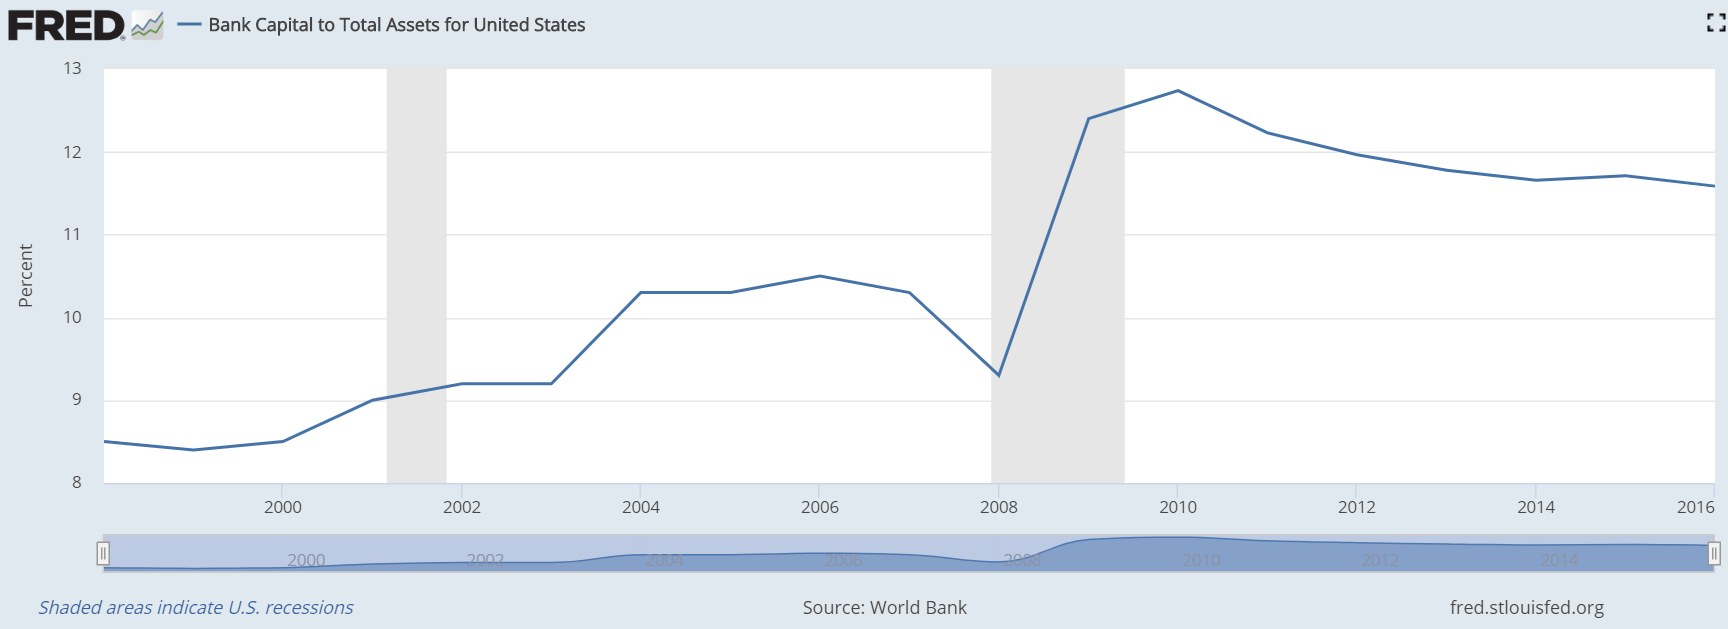
\includegraphics{Figures/US_bank_capital_asset_ratio.png}
}

\caption{\label{fig:L4_US_bank_capital_asset_ratio} Ratio of bank capital and reserves to total assets - variation over time. Source: \href{https://fred.stlouisfed.org/series/DDSI03USA156NWDB}{St Louis Fed. FRED database}}
%Capital and reserves include funds contributed by owners, retained earnings, general and special reserves, provisions, and valuation adjustments. Capital includes tier 1 capital (paid-up shares and common stock), and total regulatory capital, which includes several specified types of subordinated debt instruments which need not be repair if the funds are required to maintain minimum capital levels (these comprise tier 2 and tier 3 capital). Total assets include all nonfinancial and financial assets. 
\end{center}
\end{figure}

\end{frame}

%-------------------------------------------------------

%-------------------------------------------------------

\begin{frame}{Bank balance sheet - solvency after losses}

Suppose a bank initially has a balance sheet of size $\$100$
	\begin{itemize}
	\item	Assets:
		\begin{itemize}
		\item	$\$20$ of risky loans
		\item	$\$70$ of safe loans
		\item	$\$10$ of cash
		\end{itemize}
	\item	Liabilities:
		\begin{itemize}
		\item	$\$x$ of capital
		\item	$\$100 - \$x$ of deposits/wholesale funding/bonds
		\end{itemize}
	\end{itemize}
\vspace{2mm}
Suppose we discover that risky loans were originated under low standards
	\begin{itemize}
	\item	Learn that half are certain to default
	\item	Risky loans revalued to $\$10$
	\end{itemize}
\vspace{2mm}
Importance of initial capital
	\begin{itemize}
	\item	$x=20$ $\Rightarrow$ bank still solvent (capital reduced to $\$10$ but absorbs loss)
	\item	$x=5$ $\Rightarrow$ bank now insolvent (capital is exhausted, assets ($\$90$) $<$ liabilities ($\$95$))
	\end{itemize}

\end{frame}

%-------------------------------------------------------

%-------------------------------------------------------

\begin{frame}{Bank balance sheet - solvency problem}

\begin{figure}
\begin{center}

\resizebox{0.40\textwidth}{!}{%
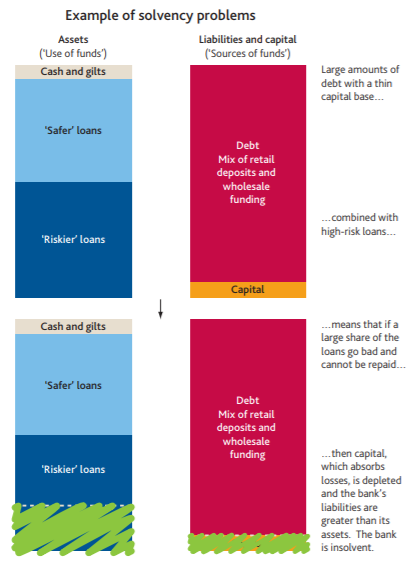
\includegraphics{Figures/bank_bs_solvency_problem.png}
}

\caption{\label{fig:L4_bank_bs_solvency_problem} Simplified bank balance sheet - example of solvency problem. Source: \href{https://www.bankofengland.co.uk/-/media/boe/files/quarterly-bulletin/2013/bank-capital-and-liquidity.pdf}{Bank of England - Farag (2013)}}

\end{center}
\end{figure}

\end{frame}

%-------------------------------------------------------

%-------------------------------------------------------

\begin{frame}{Bank balance sheet - bad loans}

\begin{figure}
\begin{center}

\resizebox{0.90\textwidth}{!}{%
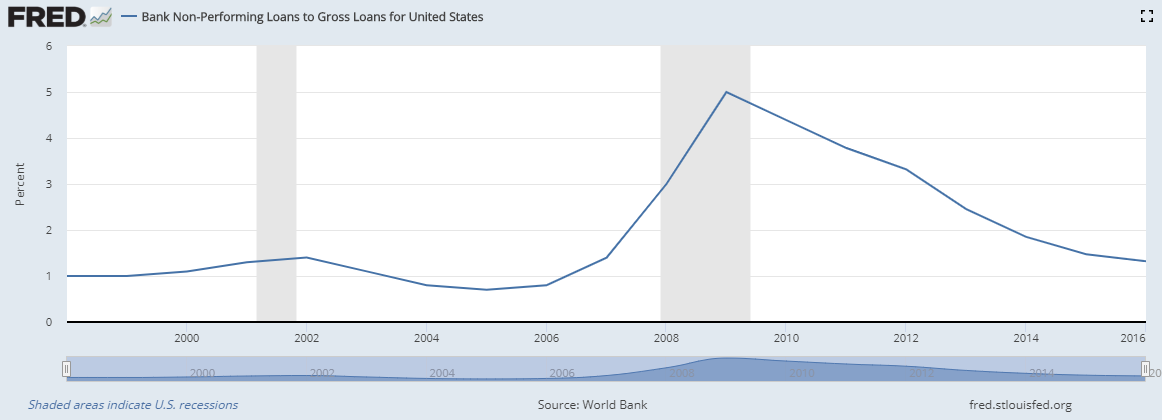
\includegraphics{Figures/NPL_to_total_loans.png}
}

\caption{\label{fig:L4_NPL_to_total_loans} Ratio of defaulting loans (payments of interest and principal past due by 90 days or more) to total gross loans (total value of loan portfolio). Source: \href{https://fred.stlouisfed.org/series/DDSI02USA156NWDB}{St Louis Fed. FRED database}}

\end{center}
\end{figure}

\end{frame}

%-------------------------------------------------------

%-------------------------------------------------------

\begin{frame}{Amplification through leverage}

Why lever up so much?
\vspace{1.5mm}
	\begin{itemize}
	\item	Consider simple example
		\begin{itemize}
		\item	$\$A$ of assets
		\item	$\$x$ of capital (or `equity')
		\item	$\Rightarrow$ `leverage ratio' of $\mathcal{L}=A/x$
		\end{itemize}
	\item	Suppose change in value of assets of $\delta$
		\begin{itemize}
		\item	Shareholders only put up $x$
		\item	Return on their equity is $\frac{\delta}{x}=\frac{A}{x}\frac{\delta}{A}=\mathcal{L}\frac{\delta}{A}$
		\end{itemize}
	\end{itemize}
\vspace{2mm}
Leverage blows up gains (but also amplifies losses)
	\begin{itemize}
	\item	People use the term `capital structure' to refer to the split between `debt' and `equity' in funding
	\item	Leverage typically thought of as total assets / equity
	\end{itemize}
	
\end{frame}

%		\begin{itemize}
%		\item	Bank managers may have short term RoE incentives
%		\item	Regulatory arbitrage arising from poorly designed risk weights
%		\item	Possible anticipation of bailout / `too big to fail'
%		\item	Artificially cheap price of debt (e.g. deposit insurance)
%		\item	Securitization (and regulatory/rating agency treatment of securitized assets)
%		\item	Possible risk shifting (though mainly at low capital levels)
%		\end{itemize}

%-------------------------------------------------------

%-------------------------------------------------------

\begin{frame}{Bank RoA and RoE}

\begin{figure}
\begin{center}

\resizebox{0.90\textwidth}{!}{%
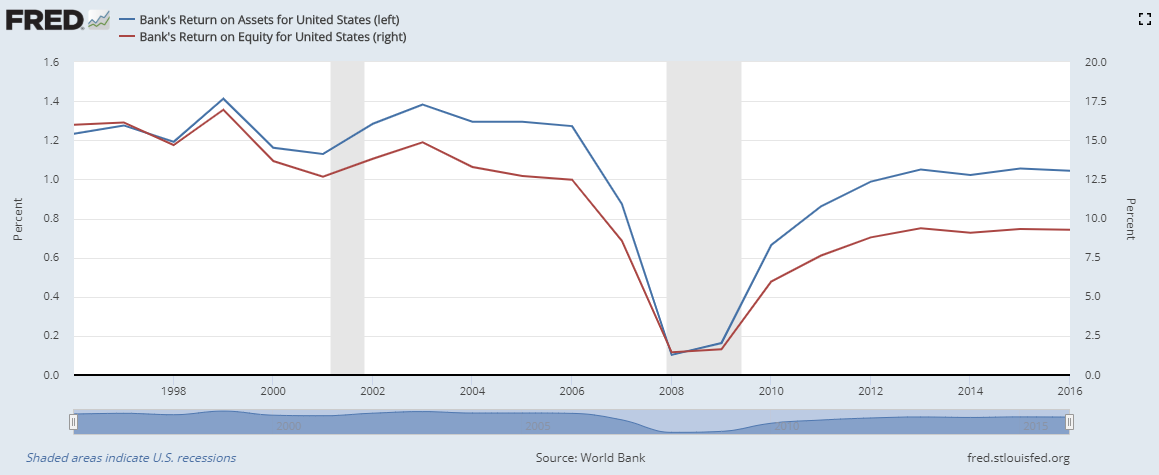
\includegraphics{Figures/roe_and_roa.png}
}

\caption{\label{fig:L4_roe_and_roa} Return on assets (percent, left scale) vs. return on equity (percent, right scale) Source: St Louis Fed. FRED database}

\end{center}
\end{figure}

\end{frame}

%-------------------------------------------------------

%-------------------------------------------------------

\begin{frame}{Models of the importance of capital}

In a perfect world the value of a firm shouldn't depend on capital structure
	\begin{itemize}
	\item	Punchline of the (in)famous \href{https://en.wikipedia.org/wiki/Modigliani\%E2\%80\%93Miller_theorem}{`Modigliani-Miller'} result
	\item	Reallocating payoffs among debt or equity holders shouldn't, \emph{per se}, change value of firm
	\item	Only overall payoff stream from a firm's activity should influence value
	\item	$\Delta$Leverage $\Rightarrow$ $\Delta$Riskiness of debt vs. equity $\Rightarrow$ $\Delta$Prices of debt vs. equity $\Rightarrow$ No $\Delta$Value of firm
	\end{itemize}
\vspace{2mm}
This result holds only in the simplest models and anecdotally there is strong disgareement with it
	\begin{itemize}
	\item	Disagreement may be self-serving (short termist bank managers may want to boost their pay in the short term)
	\item	Strong empirical evidence $\Delta$ equity affects cost of finance	
	\item	Taxes and other (typically information) frictions break the result
	\item	\textbf{Payoffs can depend on capital structure}
	\end{itemize}
	
\end{frame}

%-------------------------------------------------------

%-------------------------------------------------------

\begin{frame}{Models of the importance of capital}

Naive view of credit: If savers have funds to lend, what matters is the entrepreneur's idea and nothing else
	\begin{itemize}
	\item	Either it's a good project or it's not
	\item	How it's funded (bank credit, bonds, equity - some weird type of structured finance) doesn't matter (Modigliani-Miller again)
	\end{itemize}
\vspace{2mm}
Empirical evidence and theoretical work question this
	\begin{itemize}
	\item	\textbf{Financial accelerator} models focused on non-financial firms
		\begin{itemize}
		\item	\textit{Bernanke, Gertler and Gilchrist (1999)}: lenders must pay `auditing cost' to observe a borrower's realized return
		\item	\textit{Kiyotaki and Moore (1997)}: borrowers cannot be forced to repay debts
		\end{itemize}
	\item	Asset price variation induces fluctuations in firms' net worth
	\item	Credit tightens as net worth declines 
	\item	Reduced investment demand can further suppress asset prices
	\item	Vicious circle\ldots
	\end{itemize}

\end{frame}


%-------------------------------------------------------

%-------------------------------------------------------

\begin{frame}{Models of the importance of capital}

\begin{quote}
\ldots when borrowers have little wealth to contribute to project financing, the potential
divergence of interests between the borrower and the suppliers of external funds is
greater, implying increased agency costs; in equilibrium, lenders must be compensated
for higher agency costs by a larger premium [in the lending rate]. To the extent that borrowers' net worth is procyclical (because of the procyclicality of profits and asset prices, for example), the
external finance premium will be countercyclical, enhancing the swings in borrowing
and thus in investment, spending, and production. 
\end{quote}
\begin{center}
- Bernanke, Gertler and Gilchrist (1999)
\end{center}

\end{frame}

%-------------------------------------------------------

%-------------------------------------------------------

\begin{frame}{Models of the importance of bank capital}

\begin{quote}
Traditionally, most economists have regarded the fact that banks hold capital as at best a
macroeconomic irrelevance and at worst a pedagogical inconvenience.
\end{quote}
\begin{center}
- Ben Friedman (1991)
\end{center}

\begin{quote}
The current generation of workhorse models used for monetary policy analysis typically abstract
from imperfections in financial markets. Firms and households can borrow freely at riskless
interest rates. And financial intermediaries, if they are explicitly modeled, are nothing more than
a veil.
\end{quote}
\begin{center}
- Aikman and Paustian (2006)
\end{center}

\end{frame}

%-------------------------------------------------------

%-------------------------------------------------------

\begin{frame}{Models of the importance of bank capital}

Pre-crisis treatment of `banks' in most macro models
	\begin{itemize}
	\item	Simply a conduit for funds to flow from investors to firms
	\item	State of investors and firms might matter but bank health not separately influential
	\item	Not entirely fair: see the (readable) discussion \href{https://www.jstor.org/stable/2138389}{here}
	\end{itemize}
\vspace{2mm}
Yet similar intuitions as for firms apply to banks (banks are also firms!)
	\begin{itemize}
	\item	To the extent that monitoring of firms by banks is costly and unobservable, the bank might want to shirk
	\item	Knowing this, bank investors (e.g. depositors) want bank to have \textit{`skin in the game'}
	\item	By funding their activities partly with their own money (net worth) banks benefit from good performance of loans
	\item	\textbf{Aligns bank's incentives with the interests of bank investors}
	\item	Investors willing to fund bank at a lower rate than otherwise
	\end{itemize}

\end{frame}

%-------------------------------------------------------

%-------------------------------------------------------

\begin{frame}{Models of the importance of bank capital}

Pre-crisis treatment of `banks' in most macro models
	\begin{itemize}
	\item	Simply a conduit for funds to flow from investors to firms
	\item	State of investors and firms might matter but bank health not separately influential
	\item	Not entirely fair: see the (readable) discussion \href{https://www.jstor.org/stable/2138389}{here}
	\end{itemize}
\vspace{2mm}
Yet similar intuitions as for firms apply to banks (banks are also firms!)
	\begin{itemize}
	\item	To the extent that monitoring of firms by banks is costly and unobservable, the bank might want to shirk
	\item	Knowing this, bank investors (e.g. depositors) want bank to have \textit{`skin in the game'}
	\item	By funding their activities partly with their own money (\textcolor{red}{net worth}) banks benefit from good performance of loans
	\item	\textbf{Aligns bank's incentives with the interests of bank investors}
	\item	Investors willing to fund bank \textcolor{red}{at a lower rate than otherwise}
	\end{itemize}

\end{frame}
